%
% File: chap06.tex
%
\let\textcircled=\pgftextcircled
\chapter{Functional models}
\label{chap:fm}

\newacronym{fbed}{FBED}{Functional Basis for Engineering Design}
\newacronym{ffip}{FFIP}{Funtion Failure Identification and Propagation}
\newacronym{ffdm}{FFDM}{Function Failure Design Method}
\newacronym{uffsr}{UFFSR}{Uncoupled Flow Failure State Reasoning}

\initial{A} different way of representing an engineering system is to embed it as a functional model. A functional model is a graphical representation of a system, that ties a component to a function, or a set of functions, fulfilled within the system. Function are interconnected by flows. One of the main advantage of functional modeling is its applicability in the early stages of design, when no components have been selected and the design is just a concept. Until recently, two main methods existed to create a functional method, NIST and ?. Each had their own volatile taxonomy, which limited the widespread use of this technique to other ends than system description. Stone and Wood proposed the \gls{fbed}~\cite{stone}, which reconciled sets of function and flows notably with relation to mechanical engineering design nomenclature. This common taxonomy allowed for automatic analysis methods and database maintenance, which paved the way to various risk and reliability methods based on functional models, such as \gls{ffdm}~\cite{stone2005}, \gls{ffip}~\cite{kurtoglu2007} or \gls{uffsr}~\cite{vanbossuyt2014},~\cite{ohalloran2015}.


\section{Functional model}

A FBED description of a system uses the reconciled function set and flow set to name the various functions and flows necessary within a system. Tables~\ref{tab:fbed_func} and~\ref{tab:fbed_flow} give a few example of such functions and flows. FBED is organized using three classes, primary, secondary and tertiary, each increasing the degree of specification. THose three classes cover every potential function seen in a mechanical design. It is to be noted that it still allow for some level of interpretation as to how to categorize a function or flow.

A FBED model can be compared to a RBD. They both can take various degrees of details, high-level to low-level model description. One of the advantages that FBED exhibits as opposed to RBD is that it considers explicitely the flows linking the different functions. Moreover, it does not depend on the component selection, which allow the design team to explore a larger space of possible systems. Figure~\ref{fig:fbed} show an example of a functional model applied to the present case study. One can note that the level of details can be modified. Moreoever, to simplify the drawing, the redundancies displayed by the system are not explicited as separate functions and flows. They are instead encoded within the probabilities associated with each function or flow failure propagation.

\renewcommand{\arraystretch}{1.2}
\begin{table}[t] \small
\centering
\caption{Excerpt from the functional basis reconciled function set}
\label{tab:fbed_func}
\begin{tabular}{|c|c|c|}
\hline
Class (primary)          & Secondary                 & Tertiary  \\ \hline
\multirow{4}{*}{Branch}  & \multirow{3}{*}{Separate} & Divide    \\ \cline{3-3} 
                         &                           & Extract   \\ \cline{3-3} 
                         &                           & Remove    \\ \cline{2-3} 
                         & Distribute                &           \\ \hline
\multirow{7}{*}{Channel} & Import                    &           \\ \cline{2-3} 
                         & Export                    &           \\ \cline{2-3} 
                         & \multirow{2}{*}{Transfer} & Transport \\ \cline{3-3} 
                         &                           & Transmit  \\ \cline{2-3} 
                         & \multirow{3}{*}{Guide}    & Translate \\ \cline{3-3} 
                         &                           & Rotate    \\ \cline{3-3} 
                         &                           & Allow DOF \\ \hline
\multicolumn{3}{|c|}{...}                                        \\ \hline
Support & Position &           \\ \hline
\end{tabular}
\end{table}

\begin{table}[t] \small
\centering
\caption{Excerpt from the functional basis reconciled flow set}
\label{tab:fbed_flow}
\begin{tabular}{|c|c|c|}
\hline
Class (primary)              & Secondary                    & Tertiary                         \\ \hline
\multirow{6}{*}{Material}    & Human                        &                                  \\ \cline{2-3} 
                             & Gas                          &                                  \\ \cline{2-3} 
                             & Liquid                       &                                  \\ \cline{2-3} 
                             & \multirow{3}{*}{Solid}       & Object                           \\ \cline{3-3} 
                             &                              & \multicolumn{1}{l|}{Particulate} \\ \cline{3-3} 
                             &                              & \multicolumn{1}{l|}{Composite}   \\ \hline
\multicolumn{3}{|c|}{...}                                                                      \\ \hline
Energy & Thermal &             \\ \hline
\end{tabular}
\end{table}

\begin{figure}[t]
\centering
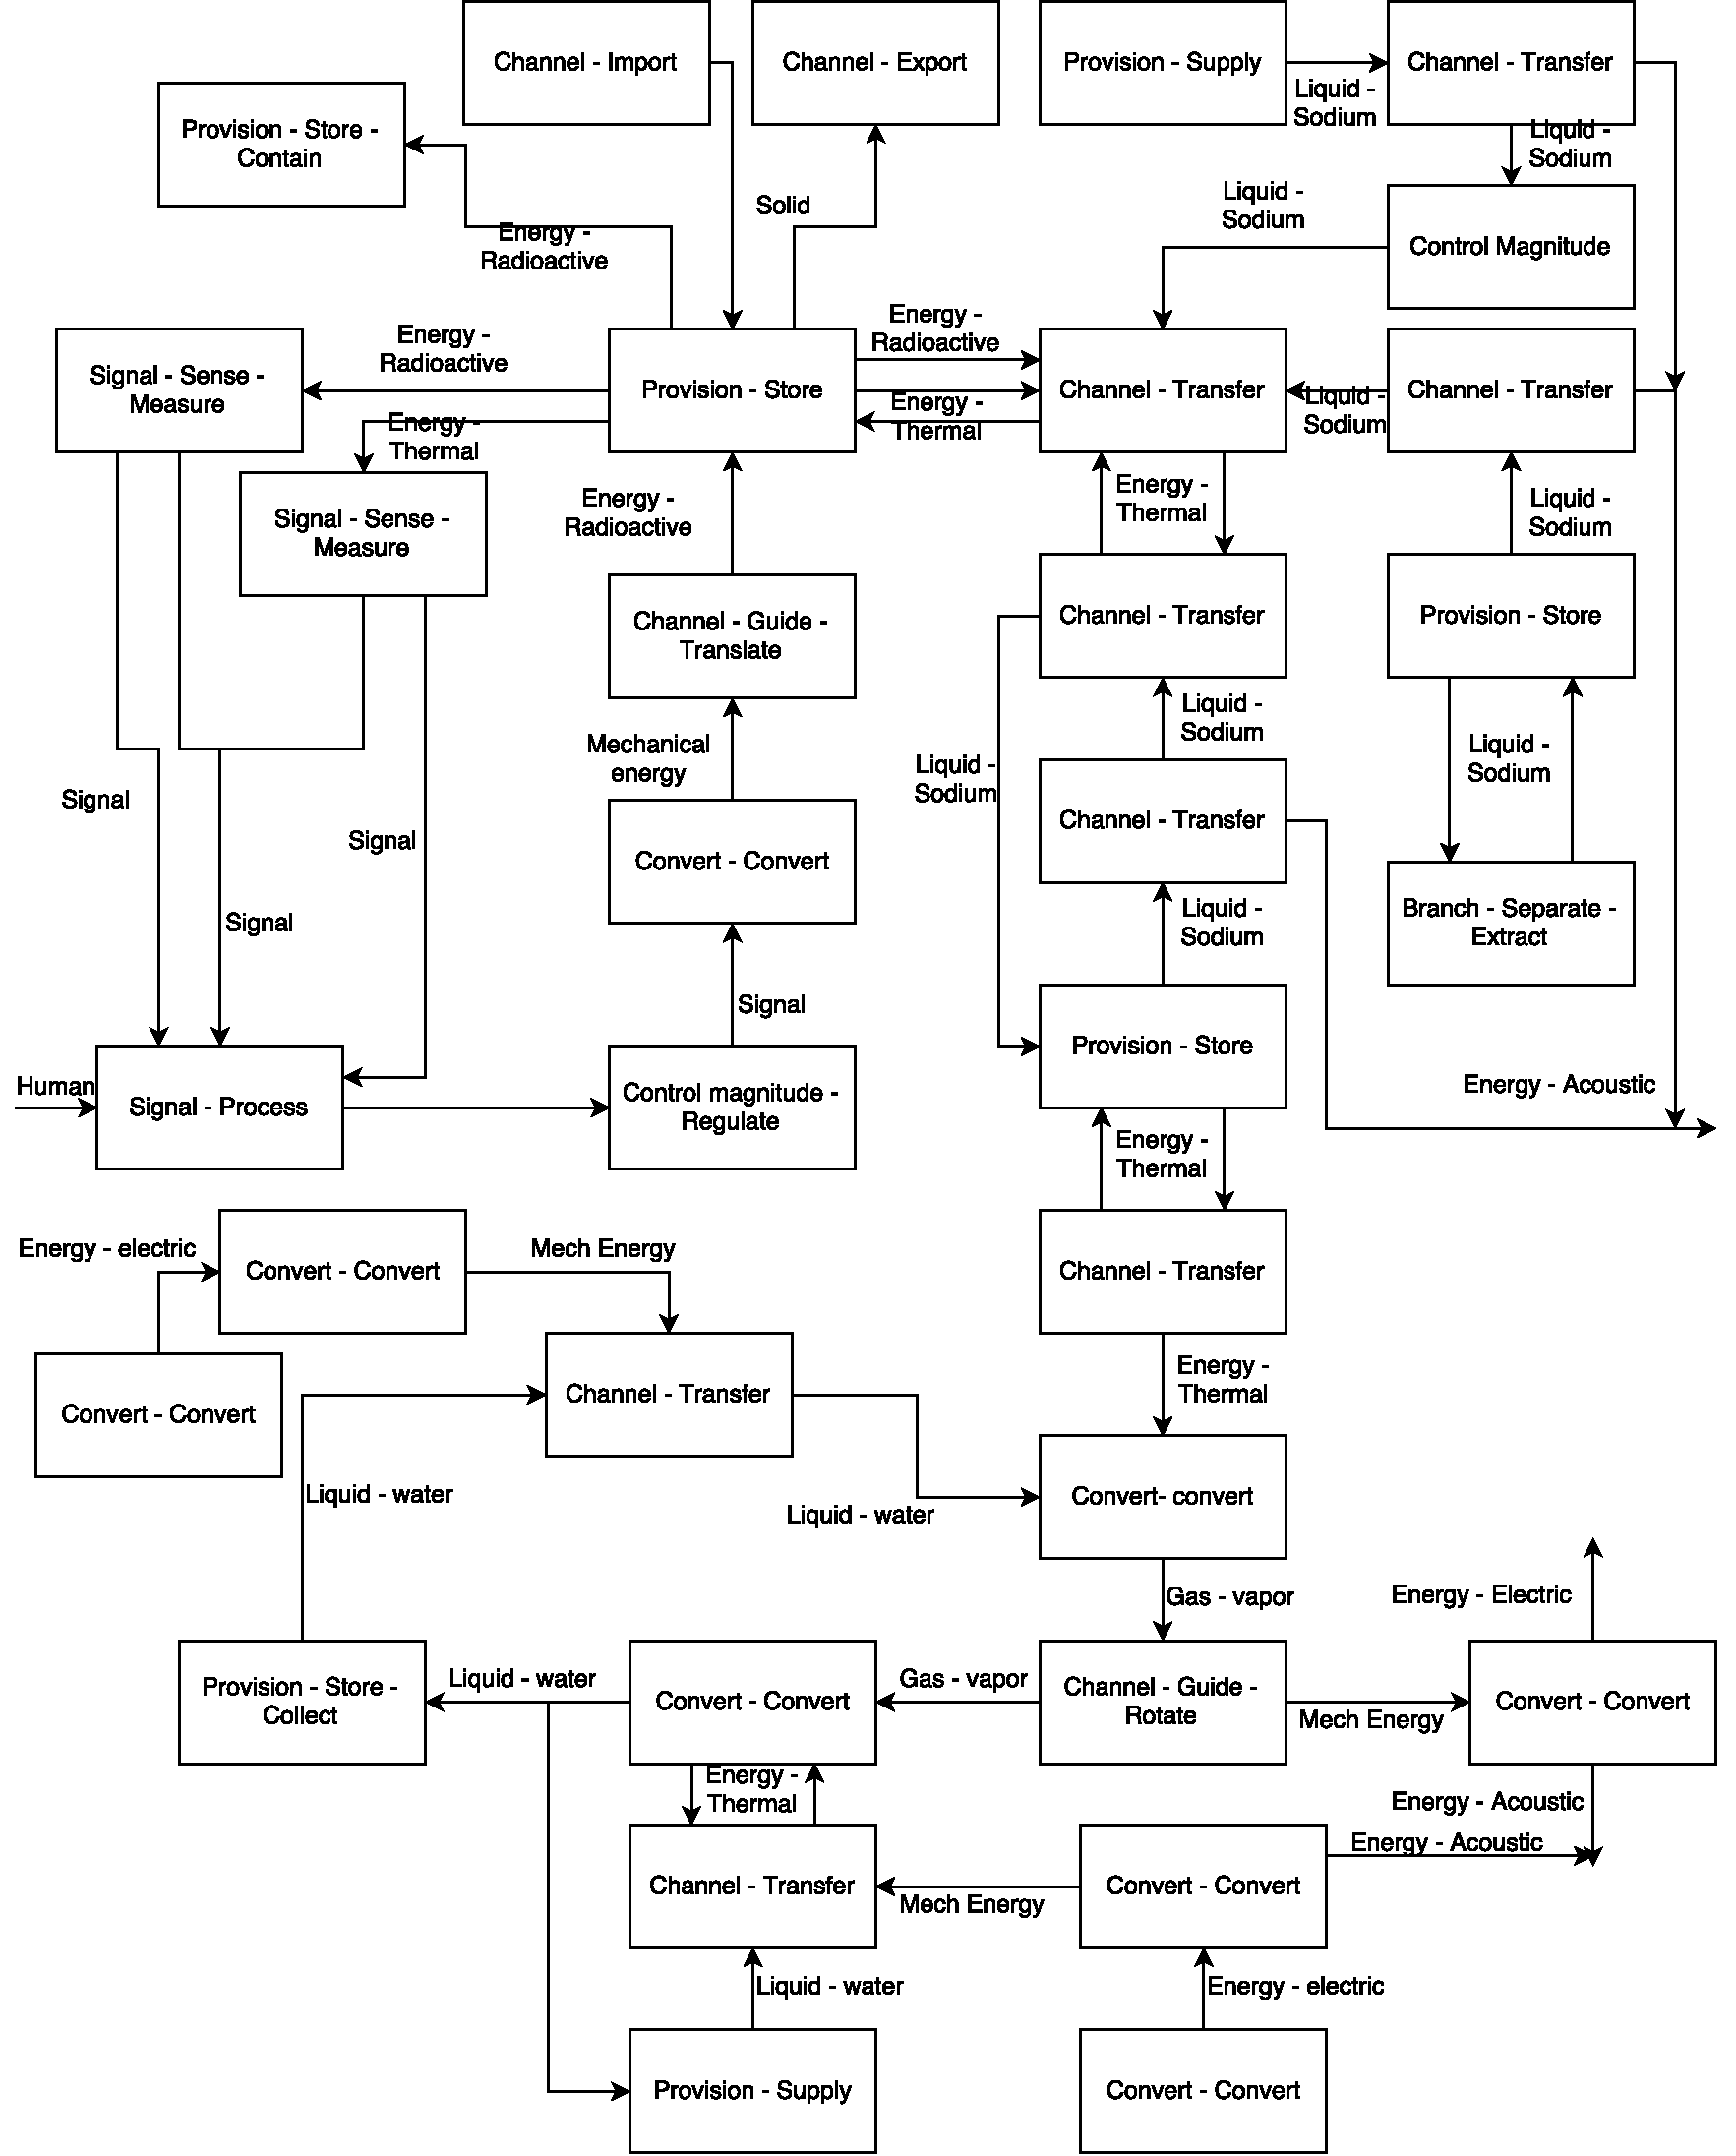
\includegraphics[scale=.6]{fig/Functional_model}
\caption{High-level simplified FBED representation of ASTRID reactor.}
\label{fig:fbed}
\end{figure}

\section{Function Failure Design Method}

FFDM is a method whose main goal is to look at historical component failure data within a system, and estimate the different failure mode observed. Those failure modes are then linked to the functions in the design. Effectively, FFDM is similar to FMEA, but allow for a more generalized approach by taking on functions. The failure modes identified can then be mitigated by modifying the functions used in the system. It has been shown that given the right database available, FFDM gave more information on the potential risk and possible actions to mitigate them in a system than FMEA. Moreover, being based on functions-failure-modes database, this method is less likely to depend uniquely on expert opinion.

However, FFDM does not diagnose the root cause of a failure, nor does it take into account manufacturing and operating conditions. Indeed, FFDM does not differentiate various levels of stress durin operations and is very dependent on past operation data to derive information about failure modes. More importantly, FFDM does not consider the severity or the detectability of a failure mode. It only focuses on the likelihood of a failure mode for each function in the system. This is an important limitation of the methodology, since it doesn't allow the design team to make fully informed decisions.

To illustrate this method, let us assume that a repository of failure modes for a given system is available. An engineering team wants to improve upon the original design, or create a new design entirely. The first step is to translate the system to a functional black-box model. Then, for each function, the failure history is analyzed, and a susceptibility score is used to link a function to all potential failure mode. Given that information, a mitigation analysis is conducted, allowing to choose the most adequate components addressing the identified function failure modes.

The fact that this method is based upon functional model allow for its use in conceptual design. One of its limitation is the existence of a complete database, and the fact that a function can fail following different failure modes depending on operating stresses and component physical attributes.

Table~\ref{tab:ffdm_dat} shows several failure modes occurences for a subset of the case study system functions.

One of the main difficulty of the FFDM method is to populate the database. Historical data is scarcely available for components, and those components must be decomposed into a functional model in order to link failure modes and functions. The failure modes considered should be drawn from a similar system, in terms of operating range and flows, to the system being analyzed. Indeed, a function "Channel - Transfer" would exhibit very different score for each failure mode in a system in which the flow is a potent acid versus a system in which the flow is room temperature water.

In order to compute the data needed for the FFDM analysis, in the absence of meaningful historical data, the FMEA analysis results presented in Table~\ref{tab:fmea_rpn_risk} are considered. Each component was analyzed and a list of potential failure and their likelihood was obtained. The number of occurences is then computed into Table~\ref{tab:ffdm_dat}. Table~\ref{tab:ffdm_norm} presents the normalized data, computed using Equation~\ref{eq:norm}.

\begin{equation}
f_{i, n} = \frac{f_i}{\sum_j F_j}
\label{eq:norm}
\end{equation}
Where:
\begin{conditions}
f_{i, n} & Normalized failure score for the mode $i$ \\
f_{i} & Failure score for the mode $i$ \\
\sum_j F_j & Number of functions considered
\end{conditions}

An example of the methodology applied to derive FFDM database from the FMEA analysis rather than historical data is explicited on the component \textit{Fuel assemblies}. A fuel assembly can be translated into a \textit{Provision - Store - Contain} function. FMEA analysis detected five different potential failure modes: a high power peaking factor, a very high power peaking factor, a human mistake (misidentification), wear and a damage to the head. We can categorize those five failure modes into various categories. The high power peaking factors can both be put in the thermal stress category. A human mistake to misidentify a fuel assembly can be categorized as a human attack. Damage to the assembly head can be sorted into the mechanical stress category. Once the main categories are computed, the likelihood of each events are taken from the FMEA analysis and incremented to the total value for each category. In this example, it would mean that \textit{Thermal stress} has a score of 13 ($8+5$), \textit{Human attack} a score of 3, and so on.

Then, the other components exhibiting the function \textit{Provision - Store - Contain}, such as the inner vessel or the core catcher, are analyzed and their failure modes scores are added to their relevant categories.

\begin{table}[t] \tiny
\centering
\caption{FFDM database}
\label{tab:ffdm_dat}
\begin{tabular}{|c|c|c|c|c|l|c|c|c|}
\hline
Function/Failure            & \begin{tabular}[c]{@{}c@{}}Corrosion\\ Fatigue\end{tabular} & \begin{tabular}[c]{@{}c@{}}Human \\ Attack\end{tabular} & \begin{tabular}[c]{@{}c@{}}Thermal\\ Stress\end{tabular} & \begin{tabular}[c]{@{}c@{}}Mechanical\\ Shock\end{tabular} & \multirow{8}{*}{...} & \begin{tabular}[c]{@{}c@{}}Mechanical\\ Stress\end{tabular} & \begin{tabular}[c]{@{}c@{}}Radiation\\ Damage\end{tabular} & \begin{tabular}[c]{@{}c@{}}Electronic\\ Failure\end{tabular} \\ \cline{1-5} \cline{7-9} 
Channel - Transfer          & 18                                                           & 12                                                                   & 0                                                              & 8                                                       &                      & 0      & 6  & 0 \\ \cline{1-5} \cline{7-9} 
Provision - Store - Contain & 10                                                           & 14                                                                   & 13                                                              & 5                                                       &                      & 0      & 11   & 0 \\ \cline{1-5} \cline{7-9} 
Signal - Sense - Measure    & 0                                                           & 0                                                                   & 0                                                              & 0                                                       &                      & 0      & 0   & 33 \\ \cline{1-5} \cline{7-9} 
Convert - Convert           & 17                                                           & 5                                                                   & 0                                                              & 6                                                       &                      & 0      & 4   & 0 \\ \cline{1-5} \cline{7-9} 
Branch - Separate - Extract & 6                                                           & 0                                                                   & 0                                                              & 0                                                       &                      & 0      & 1   & 0 \\ \cline{1-5} \cline{7-9} 
Channel - Guide - Translate & 0                                                           & 0                                                                   & 0                                                              & 5                                                       &                      & 20      & 0   & 0 \\ \cline{1-5} \cline{7-9}
\multicolumn{9}{|c|}{...}                                                                                                                                                                                                                                                                                                    \\ \hline
\end{tabular}
\end{table}


\begin{table}[t] \tiny
\centering
\caption{FFDM normalized database}
\label{tab:ffdm_norm}
\begin{tabular}{|c|c|c|c|c|l|c|c|c|}
\hline
Function/Failure            & \begin{tabular}[c]{@{}c@{}}Corrosion\\ Fatigue\end{tabular} & \begin{tabular}[c]{@{}c@{}}Human \\ Attack\end{tabular} & \begin{tabular}[c]{@{}c@{}}Thermal\\ Stress\end{tabular} & \begin{tabular}[c]{@{}c@{}}Mechanical\\ Shock\end{tabular} & \multirow{8}{*}{...} & \begin{tabular}[c]{@{}c@{}}Mechanical\\ Stress\end{tabular} & \begin{tabular}[c]{@{}c@{}}Radiation\\ Damage\end{tabular} & \begin{tabular}[c]{@{}c@{}}Electronic\\ Failure\end{tabular} \\ \cline{1-5} \cline{7-9} 
Channel - Transfer          & 4.5                                                           & 3                                                                   & 0                                                              & 2                                                       &                      & 0      & 1.5  & 0 \\ \cline{1-5} \cline{7-9} 
Provision - Store - Contain & 2                                                           & 2.8                                                                   & 2.6                                                              & 1                                                       &                      & 0      & 2.2   & 0 \\ \cline{1-5} \cline{7-9} 
Signal - Sense - Measure    & 0                                                           & 0                                                                   & 0                                                              & 0                                                       &                      & 0      & 0   & 16.5 \\ \cline{1-5} \cline{7-9} 
Convert - Convert           & 4.25                                                           & 1.25                                                                   & 0                                                              & 1.5                                                       &                      & 0      & 1   & 0 \\ \cline{1-5} \cline{7-9} 
Branch - Separate - Extract & 6                                                           & 0                                                                   & 0                                                              & 0                                                       &                      & 0      & 1   & 0 \\ \cline{1-5} \cline{7-9} 
Channel - Guide - Translate & 0                                                           & 0                                                                   & 0                                                              & 5                                                       &                      & 20      & 0   & 0 \\ \cline{1-5} \cline{7-9}
\multicolumn{9}{|c|}{...}                                                                                                                                                                                                                                                                                                    \\ \hline
\end{tabular}
\end{table}

The FFDM database obtained shows that the failure mode \textit{Corrosion fatigue} is present with a high score in a number of function. This is something the design team should consider, notably when deciding what material to use and the operating conditions that it will be subject to. A very high number can be seen, the \textit{Mechanical stress} for the \textit{Channel - Guide - Translate} function. The score displayed is 20. Moreover, a score of 16.5 can be seen for the \textit{Electronic failure} of the function \textit{Signal - Sense - Measure}. This is explained by the fact that the failure mode are highly likely for the given function. It can be seen that no other function exhibit those failure modes. A particular attention should thus be ported on the two functions, whether it is redundancies or improving the system.

A crucial information is missing from this analysis. The likelihood of a failure mode damaging a function can be computed, based on historical data and even based on expert judgement if needed. However, the consequences of these failure on the system cannot be calculated. This leaves a consequent unknown out of the design team reach, since they cannot from this data alone take an informed decision. Consequently, this method can be judged unsufficient for larger complex systems, but proves useful in the context of a concept generator, to choose a component that is better than another for a given functionality. FFDM can also be used in the very early stage of design to point toward the direction to follow for the design, potentially avoiding some costly changes late in the design phase.

\section{Function Failure Identification and Propagation}

FFDM can be used to select the most adequate components for a given functionality in a system, based upon historical failure data. However, it does not show how a failure caused by one of these componenets can propagate through the system. Reliability Block diagrams can be used to calculate the failure propagation through the components of a system, but this is limited to the end stages of design, when the whole system is mapped out. It is however crucial, in terms of risk and reliability analysis as well as in terms of design costs, to be able to compute potential failure propagation in the early phase of the design. This allows the engineers to make informed decisions about risk in the system and ways to mitigate them.

By applying a propagation method to a functional model, it is possible to get some insights about the system early on. FFDM data can be used to translate historical component failure to function failure probabilities. FFIP uses this data to propagate the failure through various flows in the system after a given initializing event. Analyzing the system in such a way can reveal weak points in the design, where mitigation action could be taken at the design stage, such as adding a redundancy or redirecting a failure flow.

In the case study at hand, several failure flow propagation were studied.
